% Ramcloud Backend

\begin{figure}[t!]
\begin{center}
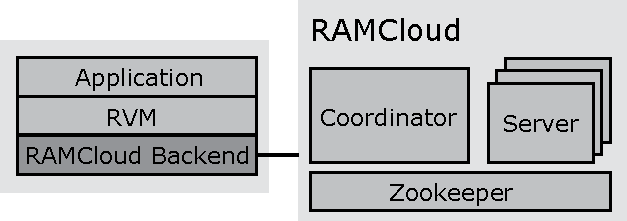
\includegraphics[scale=0.60]{graphs/ramcloud_backend_design_final.pdf}
\end{center}
\caption{RAMCloud backend layer operating along side RAMCloud.}
\label{fig:ramcloud_backend_design}
\end{figure}

\begin{figure}[t!]
\begin{center}
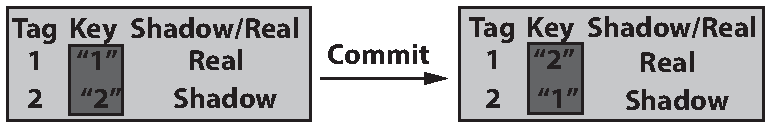
\includegraphics[scale=0.60]{graphs/ramcloud_backend_commit.pdf}
\end{center}
\caption{Diagram of tag/key mapping transformation during commit for a single memory region.}
\label{fig:ramcloud_backend_commit}
\end{figure}

To investigate the performance and suitability of a key-value store as a block device we developed a software layer on top of RAMCloud, a low-latency key-value store.
In RAMCloud, blobs of memory (values) are identified by keys (strings). When running RAMCloud is composed of three main executing instances: a coordinator, a server and Zookeeper (see Figure~\ref{fig:ramcloud_backend_design}).
Each server is responsible for storing and serving data (values). The coordinator is responsible for keeping track of all servers alive and for keeping track of where data is stored in the system.
A Zookeeper instance is used for leader election and for storing configuration data.

Because RAMCloud's data is reference by keys (string) this layer keeps a map structure that associates each tag to a key. This means that each recoverable memory region can be uniquely identified by a key.

To provide atomicity and durability of the tag/key mapping, this backend keeps a special entry in RAMCloud with each tag-key association. This table is read each time the software layer is started and written once for each commit. Because this entry can be atomically written with a {\emph put} operation, we can provide very efficient atomic writes.

Th RMEM's layer operations are implemented in the following way:

\paragraph {\bf Connect} During connection the backend creates a RAMCloud client instance that is responsible for establishing a connection to the RAMCloud server.
If this is not the first time this connection is performed, i.e., if the client is under recovery, the backend recovers each tag-key mapping.
Otherwise, this layer initializes a RAMCloud table and stores an empty master entry in the RAMCloud's server.
\paragraph{\bf Allocate} During allocation, first the backend creates a key that identifies the memory being allocated in the RAMCloud server. Secondly, RAMCloud initializes
\paragraph{\bf Write} To write a memory region (identified by a tag) the backend fetches the tag's corresponding key and issues a {\emph put } operation with that key and corresponding data.
\paragraph{\bf Read} Likewise, to read a memory region the backend issues a {\emph get} operation with the tag's corresponding key. The data read from RAMCloud is copied to the final destination.
\paragraph{\bf Commit} To perform commit, the backend constructs a new master entry where each tag points to the key of the shadow memory being committed (see Figure~\ref{fig:ramcloud_backend_commit}). Likewise, the tag for each of the shadow
memory regions is made to point to the key of the old memory region (rephrase). Once this master entry is constructed in the backend, it is written atomically to RAMCloud.
\paragraph{\bf Disconnect} To disconnect, the backend clears the main data structures (e.g., local tag-key map).

Our design is simplified by the fact that our framework only replicates data to a single node. This means that we do not have to coordinate replicas.
